Das Projektergebnis umfasst eine lauffähige Simulation und einen Prototyp.
Zum Projekt stehen alle relevanten Informationen und die im Projektziel geforderten Dokumente im DMS der WBH bereit. Die Abbildung \ref{Projektergebnis} zeigt von links nach rechts die Vision, das Simualtionsergebnis und den Prototyp.

\begin{figure}[H]
    \centering
    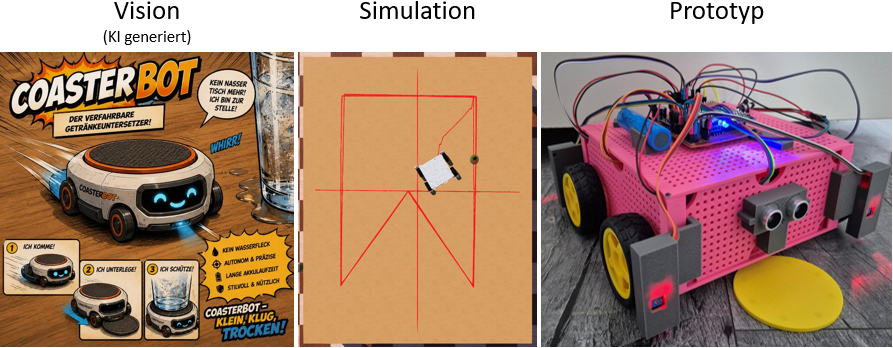
\includegraphics[width=0.9\textwidth]{Projektergebnis.png}
    \caption{Projektergebnis: Vision, Simulationsergebnis und Prototyp}\label{Projektergebnis}
\end{figure}

Damit hat das Projekt die Projektziele erreicht. Der Funktionsumfang ist jedoch kritisch zu betrachten. 
Insbesondere die Navigation und der Coastermechanismus müssen verbessert werden, um Untersetzer genauer anzufahren und zu positionieren. 
Weiterhin gibt es bisher noch keine Kontrollmechanismen, um die Anzahl der Untersetzer im Speicher zu überwachen oder eine Anwesendheit eines Untersetzer zu kontrollieren.
Damit umfasst der Prototyp lediglich Grundfunktionen, in dem er sich selbstständig bewegen, Untersetzer aufnehmen, Untersetzer ablegen und Kollisionen und Stürze vermeiden kann.